\documentclass{LabReport}
\title{计算方法数值实验3-实验报告}
\author{221900180 田永铭}
\date{\today}
\addbibresource{refs.bib}
\Chead{计算方法数值实验3-实验报告 221900180 田永铭}
\Cfoot{\thepage}
\usepackage{listings}
\usepackage{graphicx} 
\usepackage{tikzsymbols}
\usepackage{tikz}
\usepackage{hyperref}
\usepackage{amsmath}
\usepackage{amsfonts}
\usepackage{amssymb}
\usepackage{geometry}

\lstset{
	language=Matlab,               % 语言设置为Matlab
	basicstyle=\ttfamily,          % 设置等宽字体
	frame=shadowbox,               % 代码框
	showspaces=false,              % 不显示空格
	showstringspaces=false,        % 不显示字符串中的空格
	showtabs=false,                % 不显示制表符
	keywordstyle=\color{blue},     % 关键字颜色
	commentstyle=\color{green!50!black},    % 注释颜色
	stringstyle=\color{red},       % 字符串颜色
	numberstyle=\tiny\color{gray}, % 行号颜色
	rulecolor=\color{black},       % 边框颜色
	breaklines=true,               % 自动换行
	backgroundcolor=\color{white}, % 背景颜色
}

\begin{document}
	\maketitle
	
	\section{实验题目}
参考方林成森老师的《数值计算方法》上册(第二版)p183-187的算法,求解下列方程组:方程组是30×30阶的方阵。主对角线元素均为4,上下二条次对角线元素为-1,$a_{1,30} = a_{30,1} = -1$。右端向量的分量:

$f_1 = f_{30} = 6, f_2, f_3, \cdots f_{29} = 8。$方程组的形式为:

\[
\begin{bmatrix}
	d_1 & c_1 & & & & a_{1,30} \\
	a_2 & d_2 & c_2 & & & \\
	& a_3 & d_3 & c_3 & & \\
	& & \ddots & \ddots & \ddots & \\
	& & & a_{n-1} & d_{n-1} & c_{n-1} \\
	a_{30,1} & & & & a_n & d_n \\
\end{bmatrix}
\begin{bmatrix}
	x_1 \\
	x_2 \\
	x_3 \\
	\vdots \\
	x_{n-1} \\
	x_n \\
\end{bmatrix}
=
\begin{bmatrix}
	f_1 \\
	f_2 \\
	f_3 \\
	\vdots \\
	f_{n-1} \\
	f_n \\
\end{bmatrix}
\]

系数矩阵中没有标明符号的地方均为0。要求程序通用,输入系数矩阵的阶数n,系数矩阵中的非零元素,以及右端向量$\mathbf{f}$。输出:解向量$\mathbf{x}$。

	\section{实验原理}
	\begin{itemize}
		\item \textbf{实验原理——追赶法:}追赶法(也称为三对角矩阵算法或Thomas算法)是一种用于求解线性代数方程组的直接方法,特别适用于具有三对角矩阵结构的方程组。该算法通过消元和回代两个步骤来求解方程组。首先将系数矩阵进行LU分解,然后再分别解两个系数矩阵为三角矩阵的线性方程组,最终得到答案。

		\item \textbf{实验原理——变形的追赶法:}这部分原理参见林成森老师的书,主要思想是,先不看最后一个方程,将含有最后一个未知量的式子中,含有最后一个未知量的项移动到右端向量中,这样就有n-1阶形式的三对角矩阵,通过求解可以将$x_1$一直到$x_n-1$用$x_n$表示出来,再通过最后一个方程求解$x_n$,进而推导出解向量的其它项。
	\end{itemize}
	
	\section{核心代码以及说明}
	{\color{red} 本人采用了两种方法完成此次实验,一种是林成森老师的方法,一种是带着参数计算的方法,两种方法本质相同。}
	
	\subsection{林成森老师方法}
	\subsubsection{处理输入}
	
\begin{lstlisting}
n = 30; %输入周期形式三次样条的三对角矩阵维数
%输入hi,其中h1为左下角和右上角的元素,hi(i>1)为三对角两旁元素
h = double(zeros(n,1));
for i = 1 : n
    h(i) = -1;
end
%输入gi,即主对角线元素,注意主对角线元素为2*gi
g = double(zeros(n,1));
for i = 1 : n
    g(i) = 2;
end
%输入右端向量d,其中每个元素为6di,i从1到n
d = double(zeros(n,1));
d(1) = 1; d(n) = 1;
for i = 2 : n-1
    d(i) = 8/6;
end
\end{lstlisting}	
	这部分处理了输入,比较容易实现。
	
	\subsubsection{依次计算}
	根据林成森老师的方法,我们需要依次计算pk,qk,uk;sk;tk,vk;x。具体代码如下:
	
	\begin{lstlisting}
%计算pk,qk,uk
p = double(zeros(n-1,1));
q = double(zeros(n-1,1));
u = double(zeros(n-1,1));
p(1) = 2*g(1); q(1) = h(2)/p(1); u(1) = 6*d(1)/p(1);
	for k = 2: n-1
	p(k) = 2*g(k) - h(k)*q(k-1);
	q(k) = h(k+1) / p(k);
	u(k) = (6*d(k)-h(k)*u(k-1))/p(k);
end
%计算sk
s = double(zeros(n,1));
s(1) = 1;
for k = 1:n-1
	s(k+1) = -h(k)*s(k)/p(k);
end
%计算tk,vk
t = double(zeros(n,1));
v = double(zeros(n,1));
t(n) = 1; v(n) = 0;
for k = n-1:-1:1
	t(k) = -q(k)*t(k+1) + s(k+1);
	v(k) = -q(k)*v(k+1) + u(k);
end
%计算x
x = double(zeros(n,1));
x(n) = (6*d(n)-h(1)*v(1)-h(n)*u(n-1))/
    (h(1)*t(1)+h(n)*(s(n)-q(n-1))+2*g(n));
for k = 2:n-1
	x(k-1) = t(k-1)*x(n) + v(k-1);
end
x(n-1) = u(n-1) + (s(n-1) - q(n-1))*x(n);
%输出
disp('方程组Ax=b的解x是:');
disp(x)
	\end{lstlisting}	
	
	\subsection{带着参数计算的方法}
	我还实现了另一种方法,即将$x_n$看作参数,利用matlab提供的参数计算,将$x_1,x_2\cdots x_{n-1}$利用n-1阶的三对角矩阵追赶法用$x_n$表示出来,利用最后一个方程解出$x_n$,再代出$x_1,x_2\cdots x_{n-1}$。
	
	\subsubsection{处理输入}
	限于篇幅,不展示输入部分代码。值得一提的是,为了使得实验算法更具有一般性,比如能够支持不同的n,能够使得两条次对角线元素不一定相等,进一步,系数矩阵只需要满足强对角占优就能使用,这种方法我的输入处理和计算方法更{\color{red} 具有一般性}。具体到输入,我是直接输入$A_0$矩阵和右端向量$b_0$。
	
	\subsubsection{将$x_n$视作参数并且提取出n-1阶三对角矩阵}
	\begin{lstlisting}
syms xn;%将xn先视作参数
%将n阶矩阵先转化为n-1阶三对角矩阵求解,其中xn为参数
[A,b] = transform(A0,b0,xn);
%经过以下函数处理后,A,b为n-1阶的三对角矩阵系数和右端向量
function [A,b] = transform(A0,b0,xn)
    n = size(A0, 1);
    A = sym(zeros(n-1,n-1));
    for i = 1 : n-1
        for j = 1 : n-1
            A(i,j) = sym(A0(i,j));
        end
    end
    b = sym(zeros(n-1,1));
    for i = 1 : n-1
        b(i) = sym(b0(i));
    end
    b(1) = b(1) - A0(1,n)*xn; b(n-1) = b(n-1) - A0(n-1,n)*xn;
end
	\end{lstlisting}
	
	\subsubsection{n-1阶三对角矩阵的LU分解}
		\begin{lstlisting}
%以下全部算法完全来自课本
function [L, U] = lu_tridiagonal(A)
    n = size(A, 1);
    L = double(zeros(n));
    U = double(zeros(n));
    L(1,1) = A(1,1);
    U(1,1) = 1;
    U(1,2) = A(1,2) / L(1,1);
    for i = 2:n-1
        L(i, i-1) = A(i,i-1);
        L(i,i) = A(i,i) - A(i,i-1)*U(i-1,i);
        U(i,i) = 1;
        U(i,i+1) = A(i,i+1) / (A(i,i) - A(i,i-1)*U(i-1,i));
    end
    L(n, n-1) = A(n,n-1);
    L(n,n) = A(n,n) - A(n,n-1)*U(n-1,n);
    U(n,n) = 1;
end
	\end{lstlisting}

	\subsubsection{追赶法求解}
	\begin{lstlisting}
function x = solve_lu_tridiagonal(U,xn,A,b,A0,b0)
    n = length(b); y = sym(zeros(n, 1)); x = sym(zeros(n, 1));
    % 前向替代解决 Ly = b
    y(1) = b(1)/A(1,1);
    for i = 2:n
        y(i) = (b(i)-A(i,i-1)*y(i-1)) / (A(i,i)-A(i,i-1)*U(i-1,i))
    end
    % 回代解决 Ux = y
    x(n) = y(n);
    for i = n-1:-1:1
        x(i) = y(i) - U(i,i+1)*x(i+1);
    end
    n = n + 1;
    % 至此x(1)到x(n-1)已经完全转化成了x(n)的表达式
    eqn = A0(n,1)*x(1) + A0(n,n-1)*x(n-1) + A0(n,n)*xn == b0(n);
    % 使用 solve 函数求解方程,解 xn
    sol = solve(eqn, xn);
    %将x(1)到x(n-1)中的xn代成具体解
    x = subs(x, xn, sol); %将解得的xn的具体数值代回x其它分量
end
	\end{lstlisting}

\section{实验结果}
两种方法结果一致,最终计算得到的解向量如下图所示({\color{red} 为了更方便看,我将x分量的序号也打印出来了}):
\begin{figure}[h!] % 设置浮动环境
	\begin{minipage}[t]{0.48\textwidth} % 左侧 minipage,宽度为页面宽度的 0.48
		\centering
		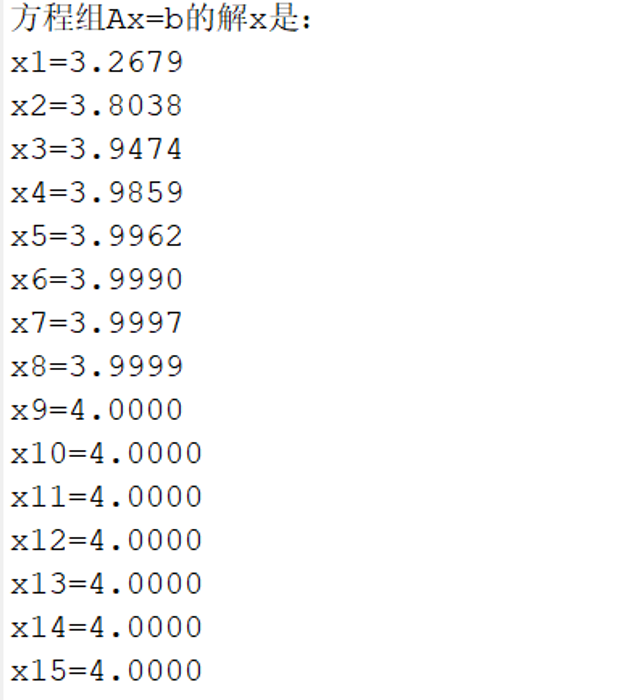
\includegraphics[width=\linewidth]{figures/3} % 插入左侧图片
		\label{fig:left_image} % 左侧图片标签
	\end{minipage}
	\hfill % 水平间距
	\begin{minipage}[t]{0.41\textwidth} % 右侧 minipage,宽度为页面宽度的 0.48
		\centering
		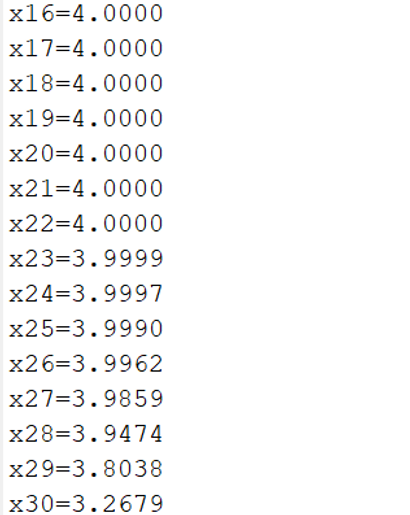
\includegraphics[width=\linewidth]{figures/4} % 插入右侧图片
		\label{fig:right_image} % 右侧图片标签
	\end{minipage}
\end{figure}

\section{总结}

\begin{enumerate}
	\item 此次实验我全部采用{\color{red} matlab}实现,全程独立实现无参考。我主动选择了使用matlab这个之前没怎么使用过的工具,了解了它的基础使用方法,并利用它完成了数值实验。
	\item 我采用了{\color{red} 两种方法}计算本次实验,其中第一种完全依据林成森老师方法,它的优点是不需要带着参数计算,纯粹是数值上的加减乘除运算,这样\textbf{效率高},缺点是不太具有一般性(林成森老师这里注重于周期三次样条得出的特定格式的三对角矩阵;当然也可以通过对公式的进一步推导使得更具有一般性);第二种方法自己探索,是带着参数进行计算,并且我注重处理了\textbf{一般性}的问题,使得任意满足强对角占优的变形的三对角矩阵都能用这个方法求解,缺点是带着参数运算效率更低。两种方法得到了一致的计算答案。
	\item 通过这次实验,我理论联系实际,将书本知识应用到程序上,激发了对计算方法这门课程的极大的兴趣。同时也明白了,数值实验是有误差的,是``差不多"的,但是做实验必须是仔细和精确到每一个细节的。同时,实验的方法也不唯一,而具有多样性,具有数学美。
\end{enumerate}

\end{document}
